% =====================================================================
%  Introduction to Deep Learning — Class 24
%  Topic (course plan): Convolution Networks
%  Subtopic (course plan): Applications: Object Detection,
%    Classification, Segmentation
%  Sources (course plan): Prince Chapter 10, Bishop Chapter 10
%
%  Class 23 built the layer and said nothing about any network.  This
%  class is about what you build with it.  The organising idea is that
%  the three tasks differ only in what the network must EMIT — one
%  label, a set of boxes with scores, or one label per pixel — and that
%  each output structure forces a different treatment of resolution.
%
%  Order: the three output structures; classification and the trunk
%  that shrinks; detection — boxes, IoU, sliding windows as
%  convolution, scales, suppression, direct prediction; segmentation —
%  a label per pixel, down and back up, unpooling and transpose
%  convolution, fully convolutional networks, the U-net.
%
%  C variant: the B deck with the two results absent from both set
%  texts removed -- the properties of IoU beyond its range (Bishop states
%  only that it lies in [0, 1]) and the rank bound on a linear decoder
%  from the bottleneck.  See _shared/PLAN_Classes23_24_25.md.
%
%  Compile:  xelatex main.tex   (run twice)
% =====================================================================
\documentclass[aspectratio=169, 11pt]{beamer}

\usetheme{metropoliscustom}

\usepackage{graphicx}
\DeclareGraphicsExtensions{.pdf,.png,.jpg}
\graphicspath{{figs/}{Class24_Applications_Detection_Segmentation/C_Textbook_Theorems_Only/figs/}}
\usepackage{amsmath, amssymb}
\usepackage{bm}
\usepackage{tikz}
\usetikzlibrary{arrows.meta, positioning, calc, decorations.pathreplacing,
                shapes.geometric, fit, backgrounds}
\tcbuselibrary{skins}

\definecolor{shc}{HTML}{341651}
\definecolor{tealc}{HTML}{1C7293}
\definecolor{dpc}{HTML}{800000}
\definecolor{accc}{HTML}{B8860B}

% ---- theorem environments -------------------------------------------
\setbeamertemplate{theorems}[numbered]
\usepackage{remreset}
\makeatletter\@removefromreset{theorem}{section}\makeatother
\renewcommand{\thetheorem}{\arabic{theorem}}
\newtheorem{lemmax}[theorem]{Lemma}
\newtheorem{propx}[theorem]{Proposition}
\newtheorem{corx}[theorem]{Corollary}
\newtheorem{defx}[theorem]{Definition}
\newtheorem{thmx}[theorem]{Theorem}

\newcommand{\bridge}[1]{%
  {\scriptsize\itshape\color{mcMuted} #1\par}\vspace{0.35em}}

\newcommand{\srcline}[1]{%
  \par\vspace{0.25em}%
  {\scriptsize\color{mcMuted}\hfill #1\par}}

\newcommand{\figsource}[1]{{\scriptsize\color{mcMuted} #1}}
\newcommand{\figcap}[2][0.90]{%
  \begin{center}\begin{minipage}{#1\textwidth}\centering
    {\scriptsize\color{mcMuted} #2}
  \end{minipage}\end{center}}

% =====================================================================
\title{Convolutional Networks}
\subtitle{Applications: Classification, Object Detection, Segmentation}
\author{Introduction to Deep Learning \ \textperiodcentered\ Class 24}
\institute{}
\date{}

\footleft{Introduction to Deep Learning}
\footright{Applications}
\titlelogos{}

\begin{document}

\maketitle

\begin{frame}{Outline}
  \tableofcontents
\end{frame}

% =====================================================================
\section{Three Tasks, Three Outputs}
% =====================================================================

\begin{frame}{From the layer to the task}
  \bridge{Class 23 built one layer and said nothing about any network.
  Today is about what you build with it, and the three tasks differ in
  one thing only: what the network must emit.}
  \vspace{0.1em}
  {\scriptsize
  \renewcommand{\arraystretch}{1.30}
  \begin{tabular}{@{}l@{\hspace{1.2em}}l@{\hspace{1.2em}}l@{\hspace{1.2em}}l@{}}
    \textbf{Task} & \textbf{Question} & \textbf{Output} & \textbf{Shape}\\
    classification & what is in the image? & one distribution & $C$\\
    object detection & what, and where? & boxes, each with a class and
      a score & $S^2(5B + C)$\\
    segmentation & what is at every pixel? & one distribution per
      pixel & $H \times W \times C$\\
  \end{tabular}}
  \vspace{0.55em}

  \begin{redhighlight}
    The output structure decides how much resolution the network may
    throw away. A label needs none of it; a label per pixel needs all
    of it back.
  \end{redhighlight}
\end{frame}

\begin{frame}{Notation for today}
  \vspace{0.35em}
  {\footnotesize
  \renewcommand{\arraystretch}{1.30}
  \begin{columns}[T, onlytextwidth]
    \begin{column}{0.49\textwidth}
      \begin{tabular}{@{}l@{\hspace{1.4em}}l@{}}
        $\mathbf{x}$ & the input image, $H \times W \times 3$\\
        $C$ & number of classes\\
        $p_c(\mathbf{x})$ & the softmax output for class $c$\\
        $\mathbf{b}$ & a box: centre $(b_x, b_y)$, size $(b_W, b_H)$\\
      \end{tabular}
    \end{column}
    \begin{column}{0.49\textwidth}
      \begin{tabular}{@{}l@{\hspace{1.4em}}l@{}}
        $S$, $B$ & grid cells per side, boxes per cell\\
        $\mathbf{M}$ & a strided convolution as a matrix\\
        $\mathbf{z}$ & a feature map inside the network\\
        $\mathbf{y}_{ij}$ & the per-pixel output at $(i, j)$\\
      \end{tabular}
    \end{column}
  \end{columns}}
  \vspace{0.55em}

  \begin{itemize}\itemsep0.24em
    \item Bishop writes the box as $\mathbf{b}$ with its centre, width
          and height; Prince describes the same five numbers for YOLO
          with a confidence added
    \item The layer operations --- stride, padding, pooling, the
          receptive field --- are those of Class 23 and are not
          re-derived
  \end{itemize}
  \srcline{Bishop \& Bishop (2024), \S10.4.1; Prince (2023), \S10.5.2.}
\end{frame}

\begin{frame}{What the output structure decides}
  \begin{center}
    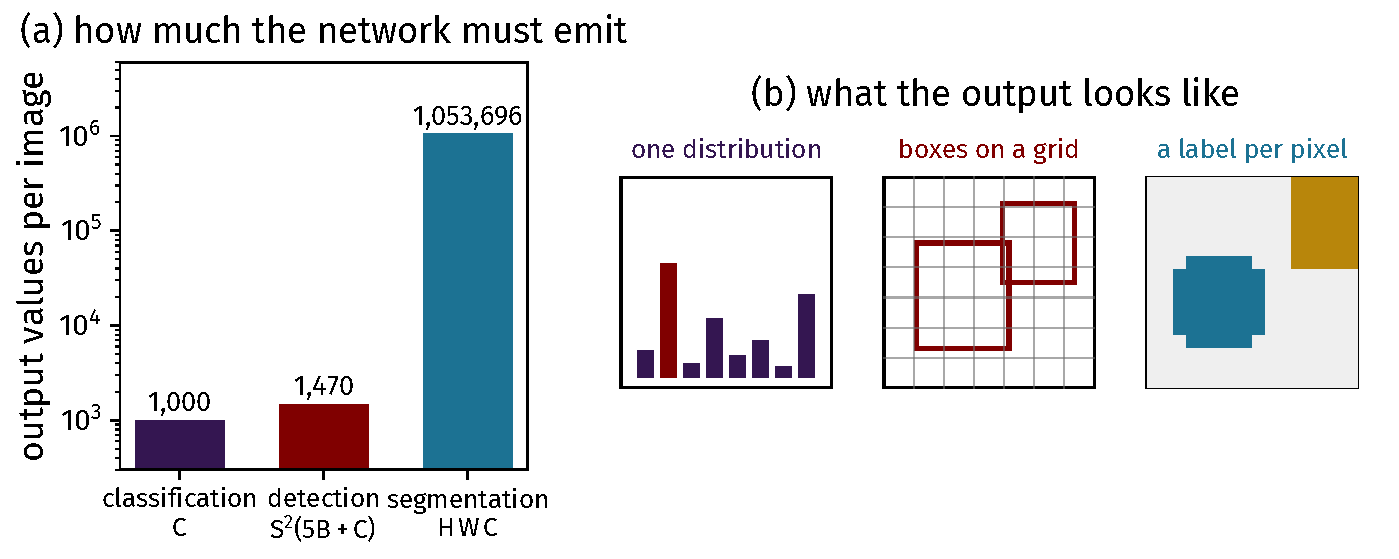
\includegraphics[width=0.90\linewidth]{output_shapes}
  \end{center}
  \vspace{-0.7em}
  {\tiny\color{mcMuted}
  (a) output values per $224 \times 224$ image, with the
  books' figures: $C = 1000$ for ImageNet; $S = 7$, $B = 2$, $C = 20$
  for YOLO; $21$ classes at each of $50{,}176$ pixels. (b) what each
  looks like.
  \hfill Prince (2023), \S10.5.1--10.5.3.\par}
\end{frame}

% =====================================================================
\section{Classification}
% =====================================================================

\begin{frame}{One label for the whole image}
  \vspace{-0.4em}
  \begin{defx}[Image classification]\label{th:cls}
    \small
    Given an image $\mathbf{x}$, emit a distribution over $C$ classes,
    \[
      p_c(\mathbf{x}) = \frac{\exp a_c(\mathbf{x})}{\sum_{c'} \exp a_{c'}(\mathbf{x})},
      \qquad c = 1, \dots, C,
    \]
    and train by the cross-entropy $-\log p_{c^\star}(\mathbf{x})$ of the
    true class. The network is a convolutional \alert{trunk} that
    shrinks the map and grows the channels, then fully connected layers
    that see the whole image at once.
  \end{defx}
  \vspace{0.05em}
  {\footnotesize
  \begin{itemize}\itemsep0.18em
    \item Translation \emph{invariance} is what is wanted here: a cat
          one pixel to the left is the same cat
    \item Pooling and the fully connected head supply it; nothing about
          \emph{where} survives to the output, by design
  \end{itemize}}
  \vspace{-0.35em}
  \srcline{Prince (2023), \S10.5.1; Bishop \& Bishop (2024), \S10.1, \S10.4.}
\end{frame}

\begin{frame}{ImageNet, the benchmark}
  \vspace{-0.25em}
  \begin{columns}[T, onlytextwidth]
    \begin{column}{0.50\textwidth}
      \vspace{0.3em}
      {\footnotesize
      \begin{itemize}\itemsep0.20em
        \item $1{,}281{,}167$ training images, $50{,}000$ validation,
              $100{,}000$ test, one of $1{,}000$ classes each, reshaped
              to $224 \times 224$ RGB
        \item Before deep networks, in 2011, the best method put the
              right class in its top five $\sim\!75\%$ of the time
        \item Within five years the best deep models had passed human
              performance
        \item Hard because the classes vary in rigidity, count,
              clutter, size, texture, colour and shape
      \end{itemize}}
      \vspace{-0.4em}
    \end{column}
    \begin{column}{0.48\textwidth}
      \begin{center}
        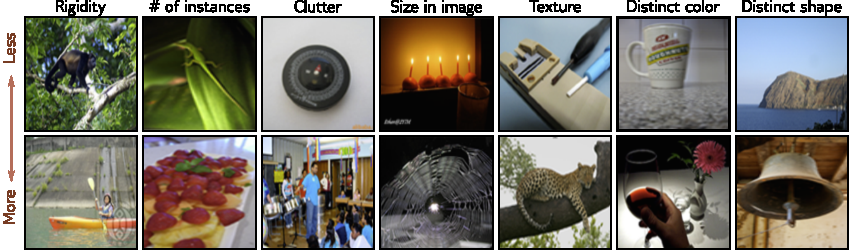
\includegraphics[width=0.82\linewidth]{P_ConvImageNet}
      \end{center}
      \vspace{-0.3em}
      \figcap[0.97]{Columns vary one attribute each. Prince (2023),
      Fig.~10.15, adapted from Russakovsky et al.\ (2015).}
    \end{column}
  \end{columns}
  \srcline{Prince (2023), \S10.5.1.}
\end{frame}

\begin{frame}{Two networks, one lesson}
  \vspace{0.1em}
  {\scriptsize
  \renewcommand{\arraystretch}{1.34}
  \begin{tabular}{@{}l@{\hspace{1.4em}}l@{\hspace{1.4em}}l@{}}
    & \textbf{AlexNet (2012)} & \textbf{VGG (2014)}\\
    hidden layers & $8$: five convolutional, three fully connected &
      $19$\\
    first layer & $11 \times 11$ kernels, stride $4$, $96$ channels &
      $3 \times 3$ kernels throughout\\
    parameters & $\sim 60$ million & $144$ million\\
    top-5 error & $16.4\%$ & $6.8\%$\\
    top-1 error & $38.1\%$ & $23.7\%$\\
  \end{tabular}}
  \vspace{0.5em}

  {\footnotesize
  \begin{itemize}\itemsep0.22em
    \item Both were trained with augmentation, dropout in the fully
          connected layers and weight decay; AlexNet with SGD, momentum
          $0.9$, batches of $128$, and five crops averaged at test time
    \item The training regimes differ in details; the change that
          mattered was \alert{depth}, and for several years deeper kept
          winning
  \end{itemize}}
  \srcline{Prince (2023), \S10.5.1; Krizhevsky et al.\ (2012);
  Simonyan \& Zisserman (2015).}
\end{frame}

\begin{frame}{Two networks, drawn to the same scale}
  \vspace{-0.2em}
  \begin{center}
    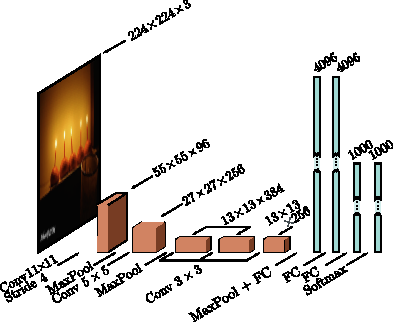
\includegraphics[height=0.40\textheight]{P_ConvAlex}\hspace{1.2em}%
    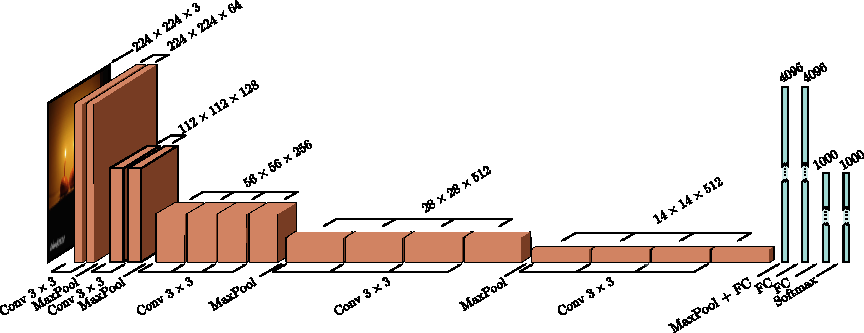
\includegraphics[height=0.40\textheight]{P_ConvVGG}%
  \end{center}
  \vspace{-0.2em}
  \figcap[0.97]{AlexNet (left) and VGG (right) at the same scale: in
  both the spatial size falls and the channel count rises along the
  trunk, and the fully connected layers come last. Prince (2023),
  Figs.~10.16 and 10.17.}
\end{frame}

\begin{frame}{Where the field went next}
  \begin{center}
    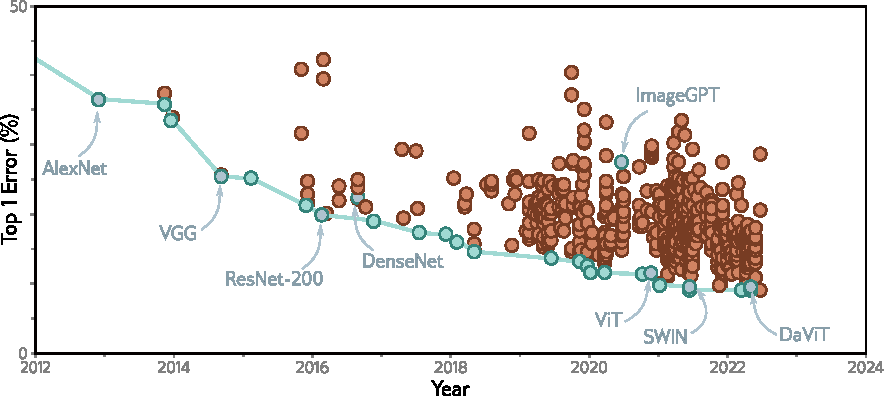
\includegraphics[width=0.66\linewidth]{P_ConvImageNetPerformance}
  \end{center}
  \vspace{-0.2em}
  \figcap[0.97]{Top-5 error on ImageNet by year; each circle is a
  published model. AlexNet and VGG were remarkable for their time; the
  residual and transformer models that overtook them are Classes 25 and
  later. Prince (2023), Fig.~10.21.}
\end{frame}

% =====================================================================
\section{Object Detection}
% =====================================================================

\begin{frame}{Where is it, and what is it}
  \vspace{-0.25em}
  \begin{defx}[Bounding box]\label{th:box}
    \small
    The location of an object is a rectangle fitting closely to it,
    \[
      \mathbf{b} = (b_x,\ b_y,\ b_W,\ b_H),
    \]
    its centre, width and height, in pixels or as fractions of the
    image with $(0, 0)$ top-left and $(1, 1)$ bottom-right. For one
    object of one of $C$ classes a network needs $C$ softmax outputs
    and four linear ones, trained by cross-entropy and a sum-of-squares
    error on $\mathbf{b}$.
  \end{defx}
  \vspace{-0.1em}
  {\footnotesize
  \begin{itemize}\itemsep0.12em
    \item Most images hold several objects, so the real problem is to
          find \alert{all} of them: the number of outputs is not known
          in advance
    \item Two families of answer: scan a classifier across the image,
          or predict boxes directly on a grid
  \end{itemize}}
  \srcline{Bishop \& Bishop (2024), \S10.4.1.}
\end{frame}

\begin{frame}{Boxes on an image}
  \begin{center}
    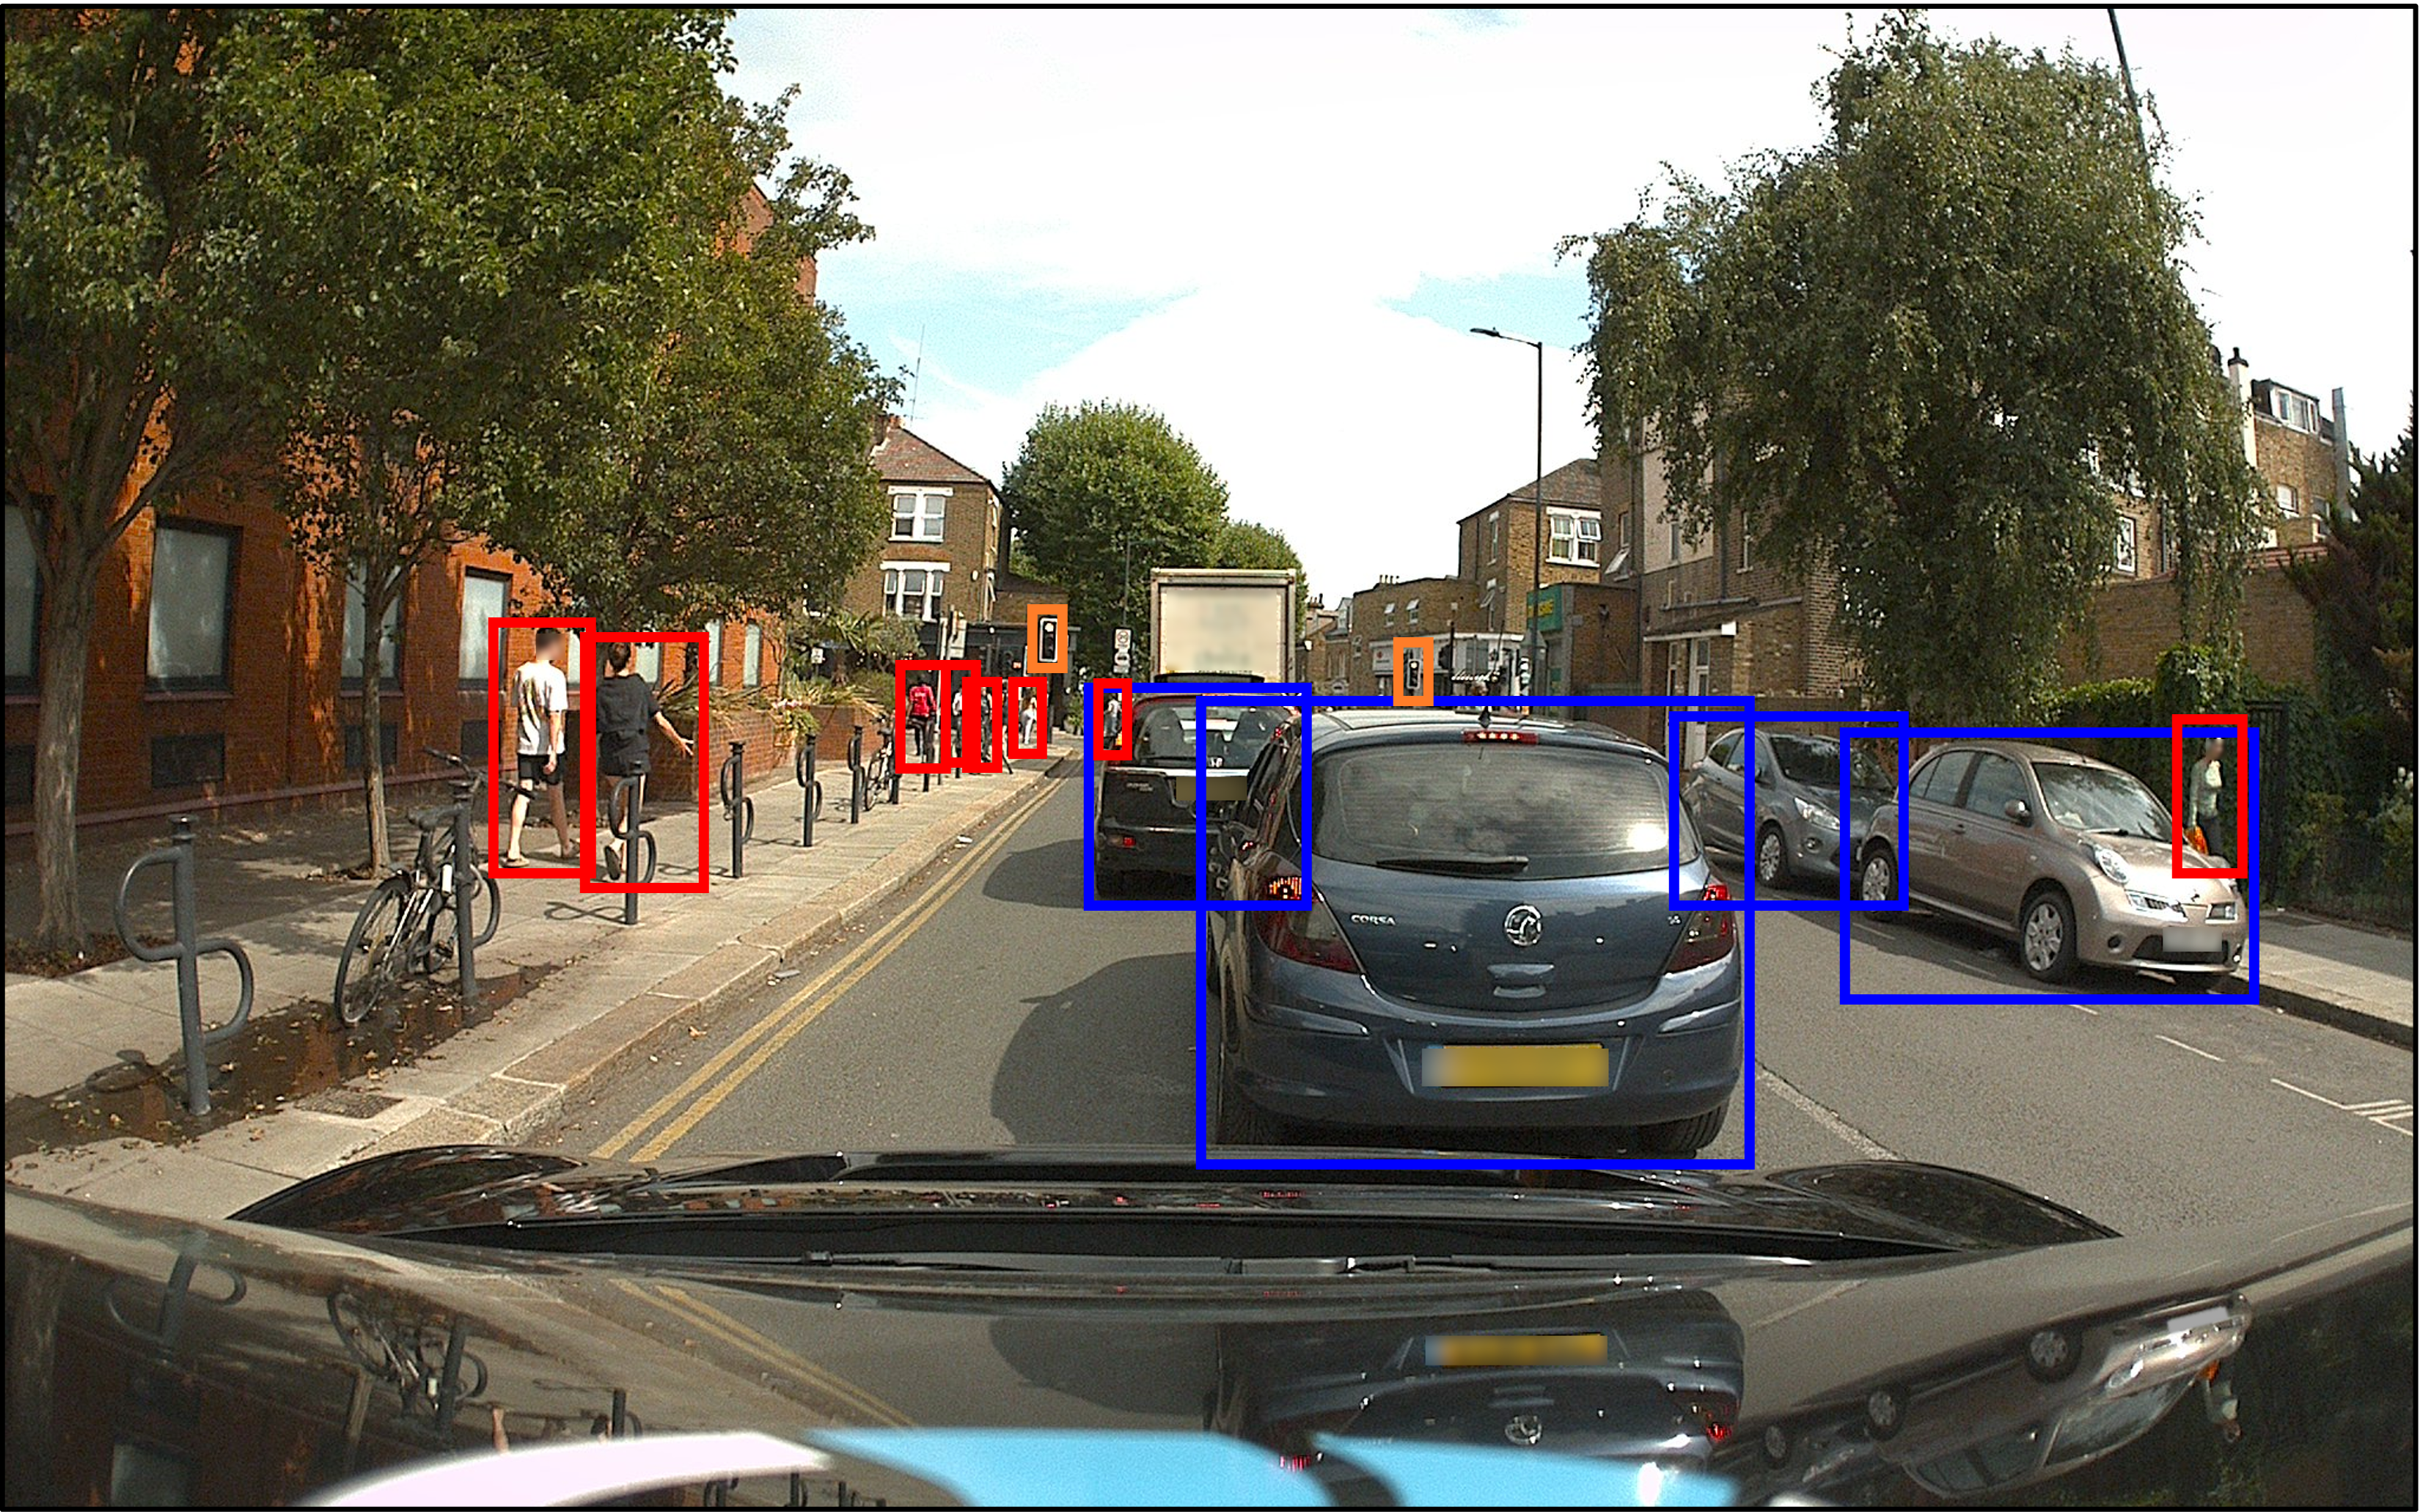
\includegraphics[height=0.56\textheight]{Bishop10_19}
  \end{center}
  \vspace{-0.2em}
  \figcap[0.97]{Every object labelled by a close-fitting rectangle;
  blue for cars, red for pedestrians, orange for traffic lights.
  Bishop \& Bishop (2024), Fig.~10.19; image courtesy of Wayve
  Technologies Ltd.}
\end{frame}

\begin{frame}{Scoring a box}
  \vspace{-0.3em}
  \begin{defx}[Intersection over union]\label{th:iou}
    \small
    For a predicted box $\mathbf{b}$ and a ground-truth box $\mathbf{b}^\star$,
    $\ \mathrm{IoU}(\mathbf{b}, \mathbf{b}^\star) =
      \mathrm{area}(\mathbf{b} \cap \mathbf{b}^\star)\,/\,
      \mathrm{area}(\mathbf{b} \cup \mathbf{b}^\star)$.
  \end{defx}
  \vspace{0.1em}
  {\footnotesize
  \begin{itemize}\itemsep0.24em
    \item The measure lies between $0$ and $1$; a prediction counts as
          correct above a threshold, usually $0.5$
    \item The overlap area alone would depend on the size of the
          object and ignore the part of the prediction outside the
          truth; the \alert{ratio} addresses both
    \item Hard to optimise by gradient descent, so it is an
          \alert{evaluation} metric; training uses centred objects
  \end{itemize}}
  \vspace{0.2em}
  \srcline{Bishop \& Bishop (2024), \S10.4.2, Fig.~10.20.}
\end{frame}

\begin{frame}{IoU, drawn and measured}
  \begin{center}
    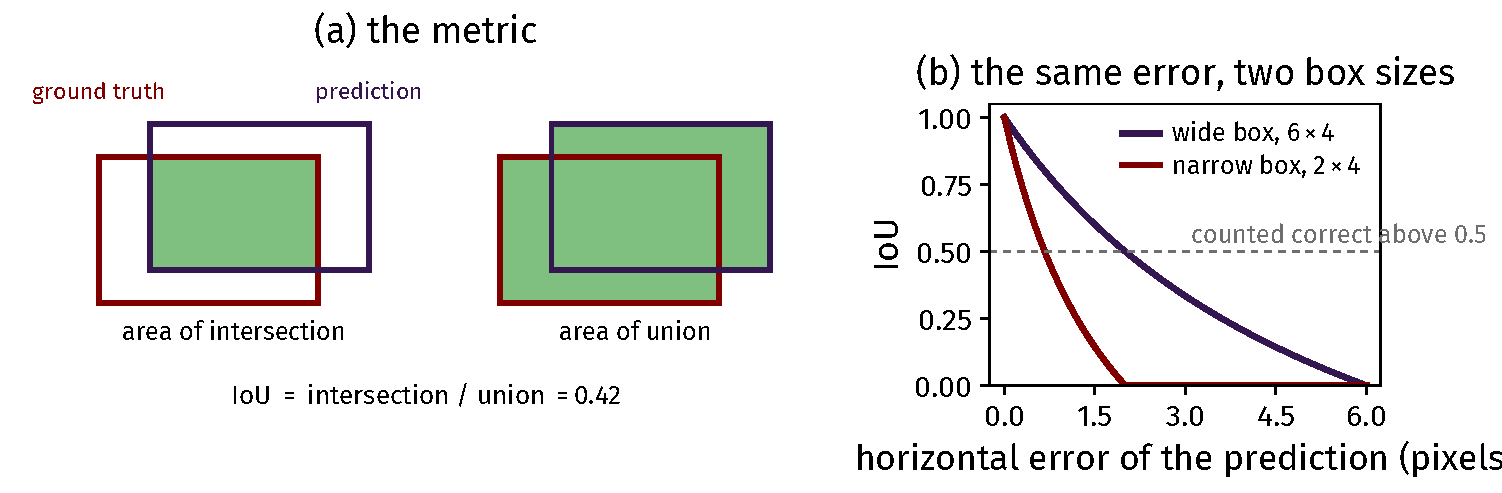
\includegraphics[width=0.92\linewidth]{iou}
  \end{center}
  \vspace{-0.7em}
  {\tiny\color{mcMuted}
  (a) the intersection and the union of a prediction and
  a ground truth, shaded, with the ratio. (b) IoU against the
  horizontal error of the prediction for a wide box and a narrow one:
  the same error in pixels costs the narrow box far more.
  \hfill Bishop \& Bishop (2024), Fig.~10.20.\par}
\end{frame}

\begin{frame}{Sliding windows}
  \vspace{0.1em}
  {\footnotesize
  \begin{itemize}\itemsep0.30em
    \item Train a classifier on tightly cropped objects and on cropped
          background; then \alert{scan} a window across a new image and
          classify each position. A confident detection makes the
          window the box
    \item The cost is the number of positions, times the cost of one
          forward pass --- prohibitive for a network of millions of
          parameters
    \item Striding the window trades precision of location for cost;
          objects of different sizes need windows of different scales
    \item But the classifier is itself a convolution sliding a detector
          across the input, so the overlapping windows repeat almost
          all of their work
  \end{itemize}}
  \srcline{Bishop \& Bishop (2024), \S10.4.3, Fig.~10.21; Sermanet et al.\ (2013).}
\end{frame}

\begin{frame}{A sliding window is a convolution}
  \vspace{-0.3em}
  \begin{propx}[Shared computation]\label{th:slide}
    \small
    Take a network of convolutions, non-overlapping poolings and one
    fully connected output, trained on $n \times n$ windows. Applied to
    a larger image with every layer enlarged accordingly, it evaluates
    all window positions in one pass: each output unit is the window
    at one position, the windows step by the product of the pooling
    factors, and the fully connected layer is a convolution whose
    kernel is the size of the pooled window.
  \end{propx}
  \vspace{0.15em}
  {\footnotesize
  \begin{itemize}\itemsep0.22em
    \item Only the units outside the first window are new work; the
          rest were computed once and reused
    \item Combining this with the direct box outputs of
          Definition~\ref{th:box} lets each window fine-tune its box
          relative to its own position
  \end{itemize}}
  \srcline{Bishop \& Bishop (2024), \S10.4.3, Figs.~10.22--10.23,
  Exercise 10.12; Sermanet et al.\ (2013).}
\end{frame}

\begin{frame}{The saving, drawn}
  \begin{center}
    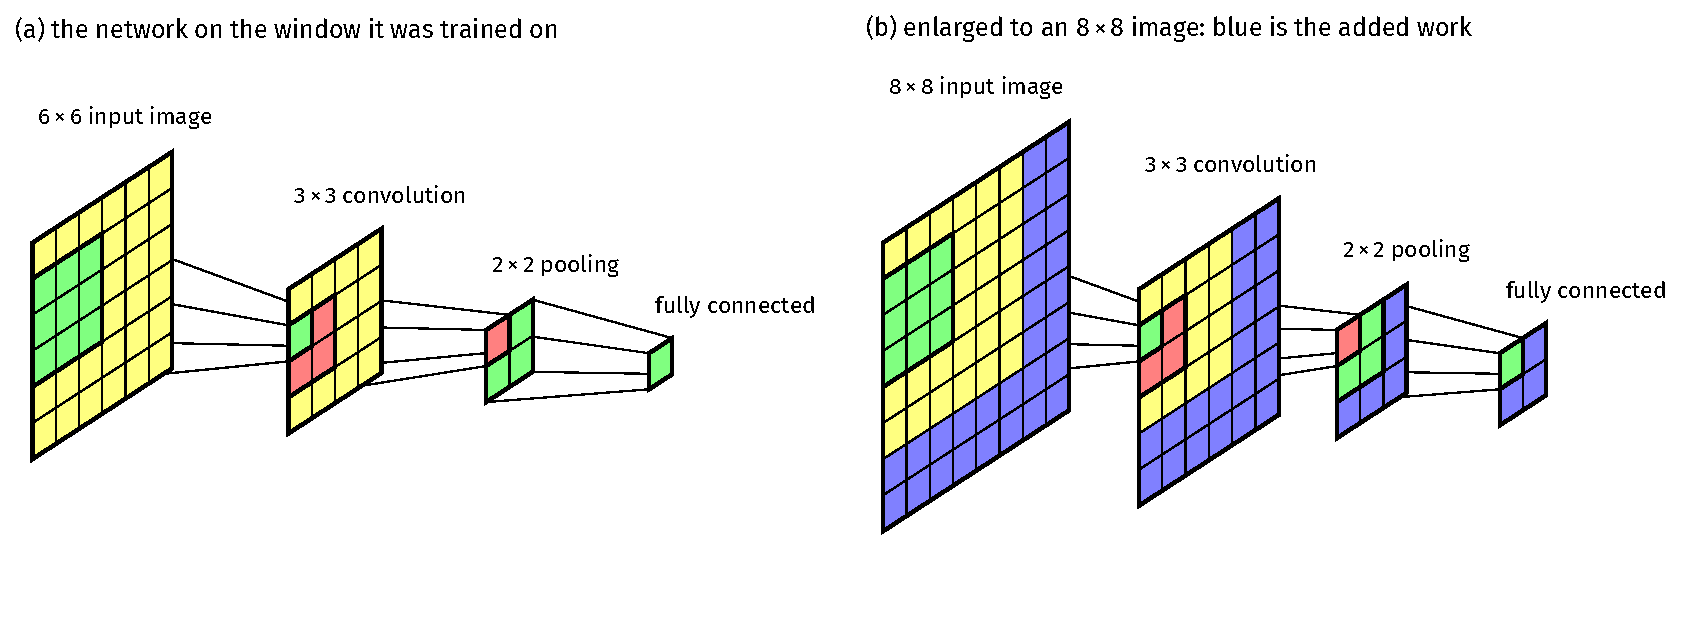
\includegraphics[width=0.92\linewidth]{sliding_window}
  \end{center}
  \vspace{-0.7em}
  {\tiny\color{mcMuted}
  (a) the toy network --- a $3 \times 3$ convolution, $2 \times 2$
  pooling and one fully connected output --- on the $6 \times 6$ window
  it was trained on; the green and red patches trace one output back
  through the layers. (b) the same network on an $8 \times 8$ image with
  every layer enlarged: four outputs, one per window position, and the
  blue cells are the only additional computation --- $340$ multiply-adds
  against $592$ for four separate passes.
  \hfill Bishop \& Bishop (2024), Figs.~10.22 and 10.23.\par}
\end{frame}

\begin{frame}{Detection across scales}
  \vspace{-0.3em}
  \begin{columns}[T, onlytextwidth]
    \begin{column}{0.50\textwidth}
      \vspace{0.3em}
      {\footnotesize
      \begin{itemize}\itemsep0.30em
        \item Objects come at every size and aspect ratio: a cat
              sitting and a cat lying down fill differently shaped boxes
        \item Instead of many windows, keep \alert{one} window and make
              many copies of the image, each scaled horizontally and/or
              vertically
        \item Scan the fixed window over every copy; when it fires,
              undo the scaling to place the box in the original image
      \end{itemize}}
    \end{column}
    \begin{column}{0.48\textwidth}
      \begin{center}
        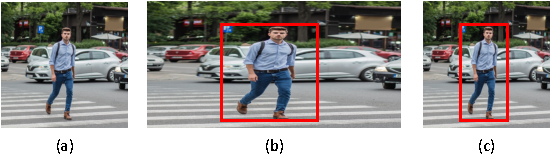
\includegraphics[width=\linewidth]{Bishop10_24}
      \end{center}
      \figcap[0.97]{(a) the image, (b) a horizontally scaled copy with
      a detection, (c) the box projected back. Bishop \& Bishop (2024),
      Fig.~10.24.}
    \end{column}
  \end{columns}
  \srcline{Bishop \& Bishop (2024), \S10.4.4.}
\end{frame}

\begin{frame}{Non-max suppression}
  \vspace{-0.25em}
  \bridge{A scanned detector fires several times around each object.
  The rule that keeps one box per object, applied one class at a time:}
  \vspace{-0.3em}
  {\footnotesize
  \begin{enumerate}\itemsep0.22em
    \item \focus{1}{Run the detector at every position and record the
          probability of the class at each.}
    \item \focus{2}{Discard every box whose probability is below a
          threshold, say $0.7$.}
    \item \focus{3}{Declare the most probable remaining box a
          detection and record it.}
    \item \focus{4}{Discard every other box whose IoU with that
          detection exceeds a threshold, say $0.5$: those are the same
          object seen again.}
    \item \focus{5}{Return to step 3 with what is left, until every
          box is either recorded or discarded.}
  \end{enumerate}}
  \vspace{-0.1em}
  \begin{redhighlight}
    Two thresholds, two meanings: the first says how sure to be, the
    second says how close is the same object.
  \end{redhighlight}
  \srcline{Bishop \& Bishop (2024), \S10.4.5, Fig.~10.25.}
\end{frame}

\begin{frame}{Suppression, drawn}
  \begin{center}
    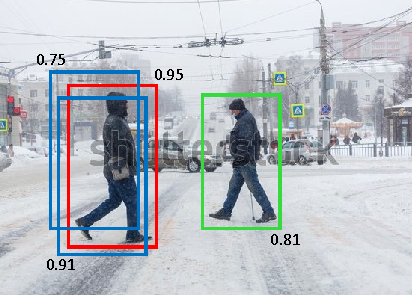
\includegraphics[height=0.50\textheight]{Bishop10_25}
  \end{center}
  \figcap[0.97]{Several detections of one object at nearby locations
  with their probabilities. The red box has the highest and is kept;
  the overlapping blue boxes are suppressed; the green box is a second
  instance and survives. Bishop \& Bishop (2024), Fig.~10.25.}
\end{frame}

\begin{frame}{Predicting boxes directly}
  \vspace{-0.3em}
  \begin{defx}[Grid prediction, YOLO]\label{th:yolo}
    \small
    Divide the image into an $S \times S$ grid. For every cell emit
    one class distribution over $C$ classes and $B$ boxes, each with
    five numbers --- $b_x, b_y, b_W, b_H$ and a confidence estimating
    the IoU with whatever object is there --- so the output is a tensor
    of size $S \times S \times (5B + C)$, produced in a single forward
    pass.
  \end{defx}
  \vspace{0.15em}
  {\footnotesize
  \begin{itemize}\itemsep0.22em
    \item In the original: a $448 \times 448$ input, $24$ convolutional
          layers shrinking to $7 \times 7 \times 1024$, a fully connected
          layer of $4096$, and one more to the output; $S = 7$, $B = 2$
    \item The trunk was first trained on ImageNet and then fine-tuned
          --- the transfer route of Class 19
    \item Low-confidence boxes are dropped and the rest pass through
          non-max suppression, exactly as before
  \end{itemize}}
  \srcline{Prince (2023), \S10.5.2, Fig.~10.18; Bishop \& Bishop (2024),
  \S10.4.1; Redmon et al.\ (2016).}
\end{frame}

\begin{frame}{Grid prediction, drawn}
  \begin{center}
    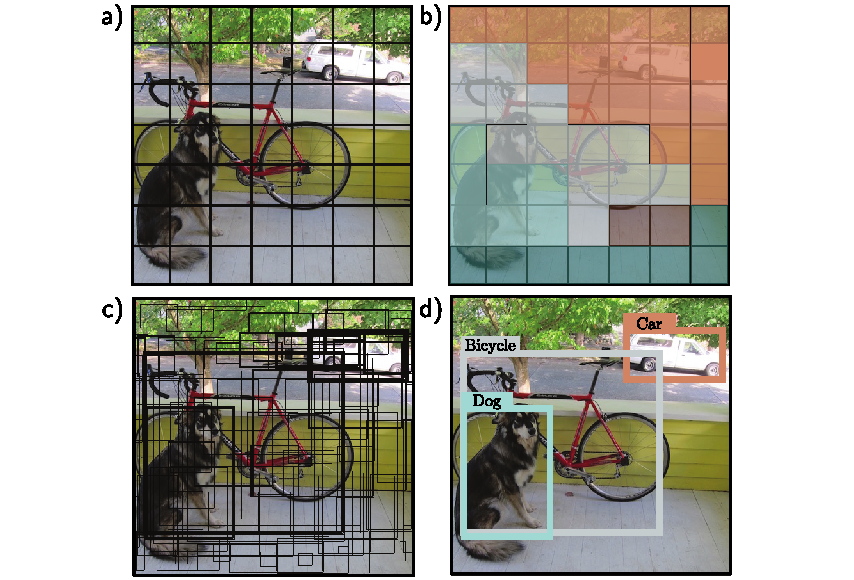
\includegraphics[height=0.56\textheight]{P_ConvYOLO}
  \end{center}
  \vspace{-0.2em}
  \figcap[0.97]{(a) the image on a $7 \times 7$ grid. (b) the most
  likely class per cell. (c) two boxes per cell with confidence as
  line thickness. (d) after suppression. Prince (2023), Fig.~10.18,
  adapted from Redmon et al.\ (2016).}
\end{frame}

\begin{frame}{Looking only where it matters}
  \vspace{0.1em}
  {\footnotesize
  \begin{itemize}\itemsep0.30em
    \item A scan spends the full network on every region, including
          those unlikely to hold anything
    \item \alert{Region proposals}: a cheap method --- a segmentation,
          say --- nominates promising regions, and the full network runs
          only there (R-CNN, fast R-CNN)
    \item Let a second convolutional network make the proposals, and
          the whole thing trains end to end (faster R-CNN)
    \item Precise localisation by scanning alone needs finely spaced
          windows; predicting the box \emph{relative to the window}
          gives the precision without the positions
  \end{itemize}}
  \vspace{0.3em}
  \begin{redhighlight}
    Every detector is some mixture of the same three ingredients: a
    classifier, a way of proposing where to look, and a box regression
    to finish the job.
  \end{redhighlight}
  \srcline{Bishop \& Bishop (2024), \S10.4.6; Girshick (2015);
  Ren et al.\ (2015).}
\end{frame}

% =====================================================================
\section{Semantic Segmentation}
% =====================================================================

\begin{frame}{A label for every pixel}
  \vspace{-0.25em}
  \begin{defx}[Semantic segmentation]\label{th:seg}
    \small
    Assign every pixel of an $H \times W$ image to one of $C$ classes.
    The output has the shape of the image with $C$ channels,
    $\mathbf{y}_{ij} \in \Delta^{C}$ for $i \leq H$, $j \leq W$,
    a softmax at each position; colouring the most probable class turns
    the prediction back into an image.
  \end{defx}
  \vspace{0.0em}
  {\footnotesize
  \begin{itemize}\itemsep0.16em
    \item This is the \alert{equivariant} task of Class 23: translate
          the input and the output must translate with it
    \item So the resolution that classification discarded on purpose
          has to be recovered, and the whole section is about how
  \end{itemize}}
  \srcline{Bishop \& Bishop (2024), \S10.5; Prince (2023), \S10.5.3.}
\end{frame}

\begin{frame}{Segmentation, on an image}
  \vspace{-0.2em}
  \begin{center}
    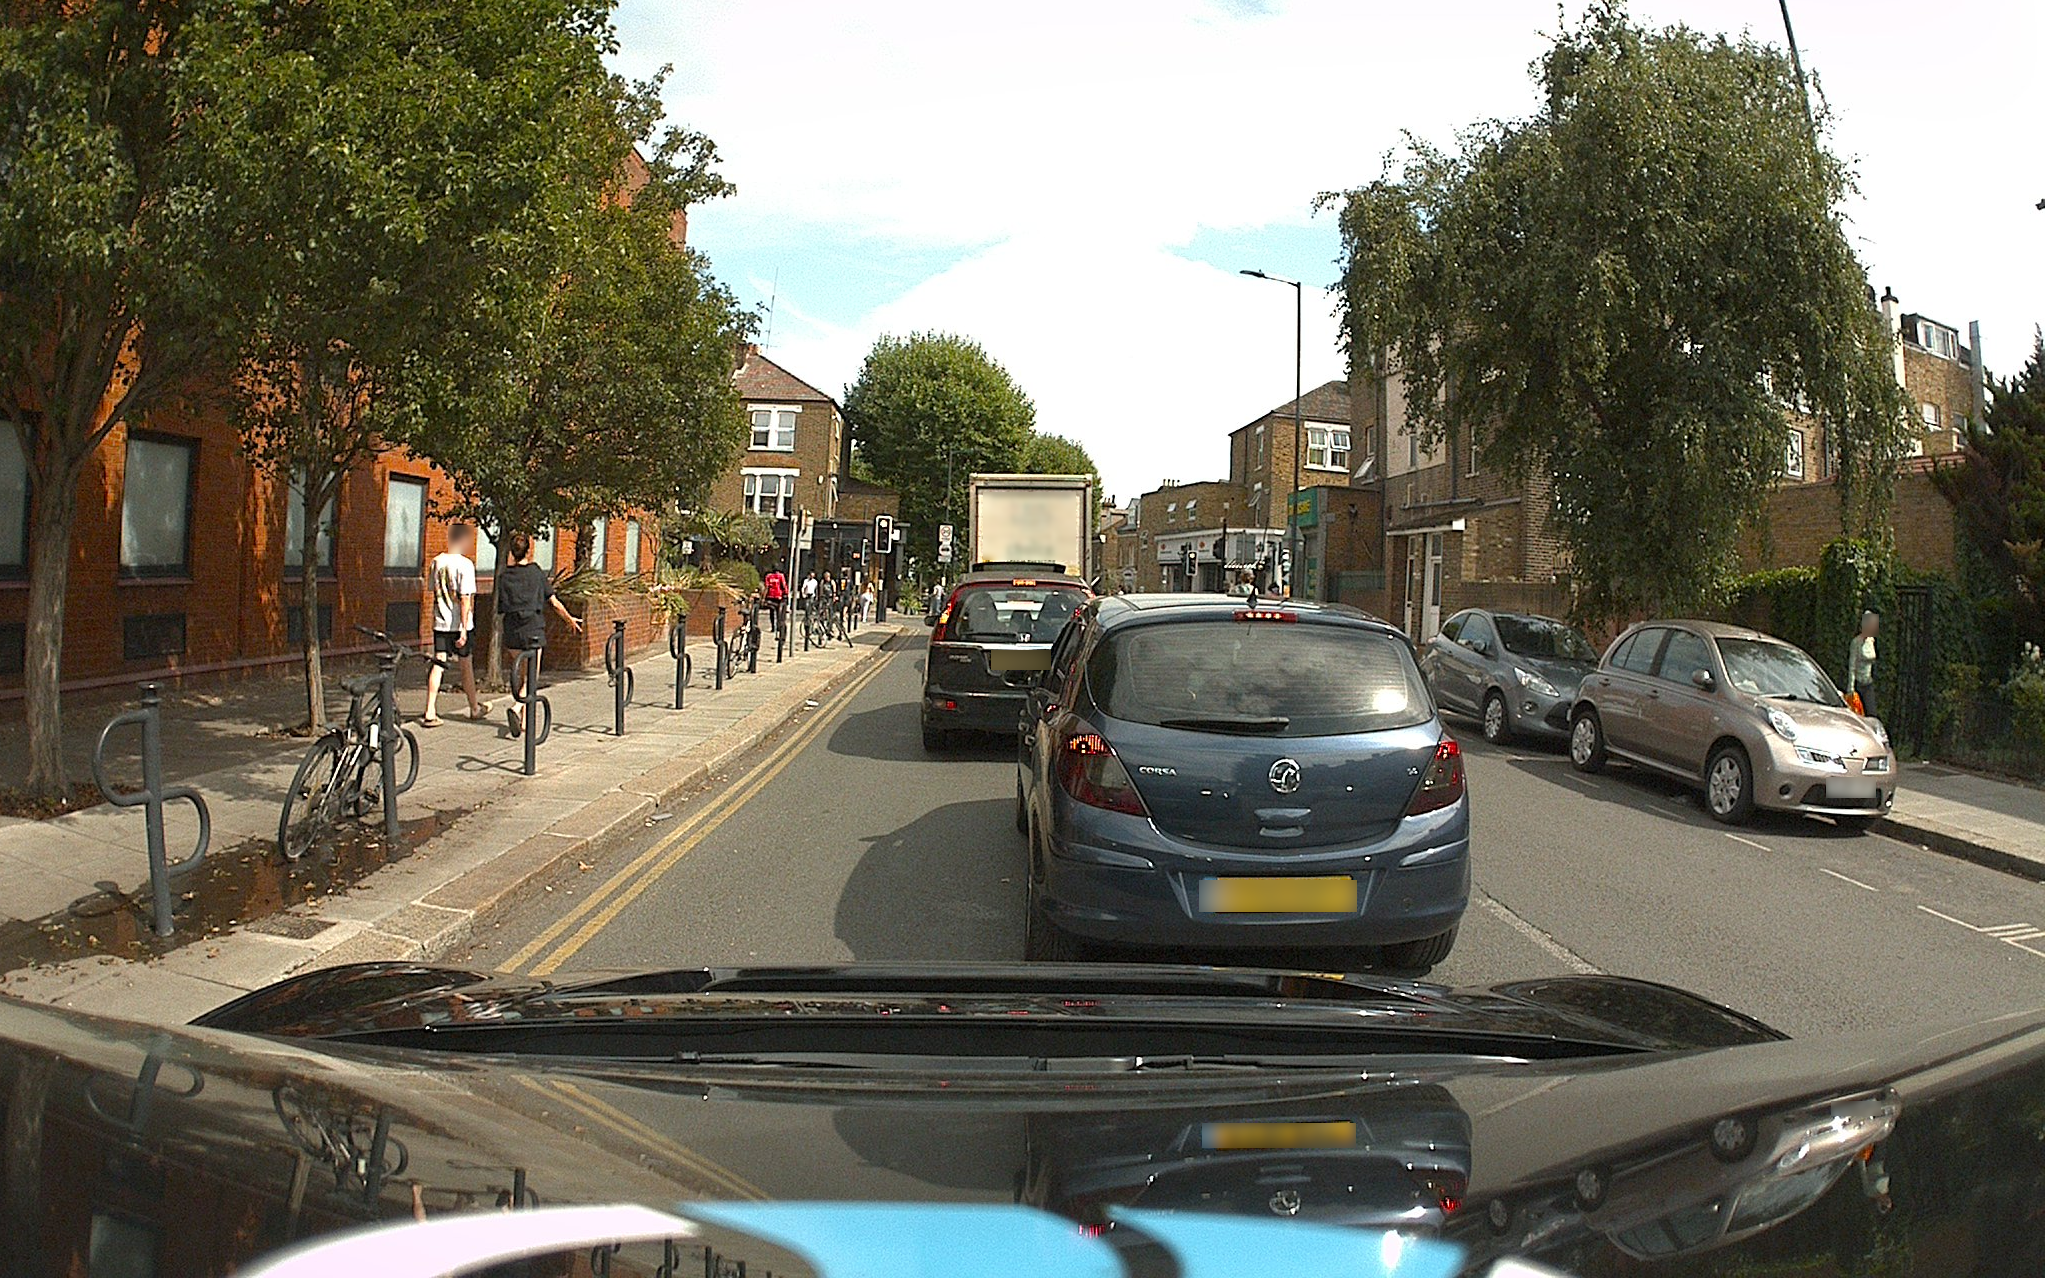
\includegraphics[height=0.42\textheight]{Bishop10_26a}\hspace{0.8em}%
    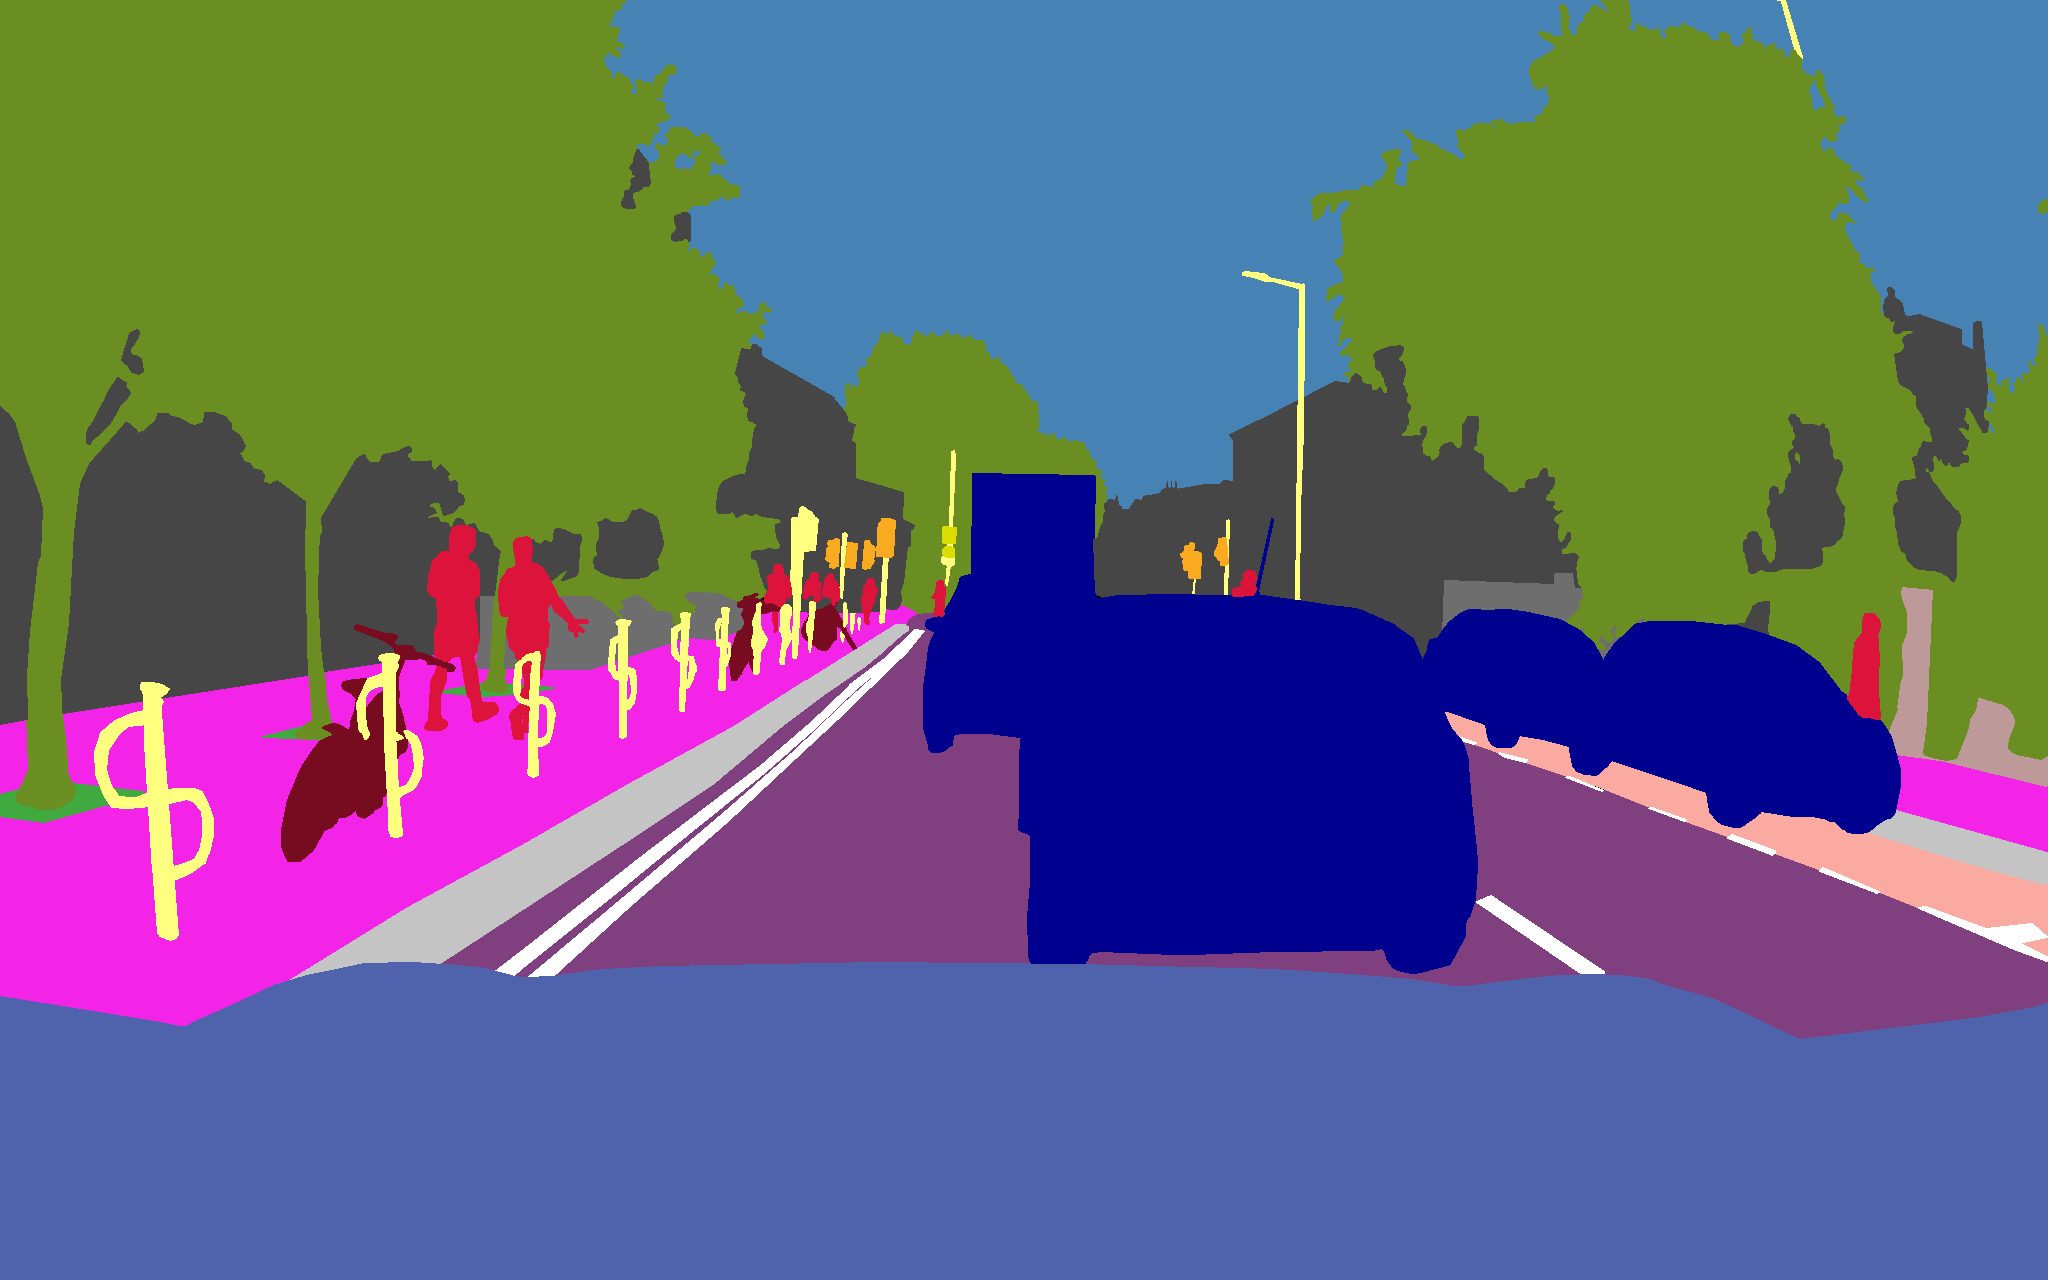
\includegraphics[height=0.42\textheight]{Bishop10_26b}%
  \end{center}
  \vspace{-0.2em}
  \figcap[0.97]{An image and its segmentation, each pixel coloured by
  class: blue for car, red for pedestrian, orange for traffic light.
  Bishop \& Bishop (2024), Fig.~10.26; courtesy of Wayve Technologies
  Ltd.}
\end{frame}

\begin{frame}{The naive network, and why it fails}
  \vspace{0.1em}
  {\footnotesize
  \begin{itemize}\itemsep0.30em
    \item Classify each pixel from a window centred on it, one forward
          pass per pixel: correct, and hopelessly redundant, since
          neighbouring windows overlap almost entirely
    \item Proposition~\ref{th:slide} removes the redundancy: one network
          whose every layer has the size of the image, stride one,
          same padding, no pooling, a shared softmax at every output
    \item That network has no way to shrink, so every layer carries a
          full-resolution map with many channels, and for a real image
          the cost is prohibitive
    \item The classification trunk solved cost by \alert{pooling}; the
          question is how to pool and still answer at every pixel
  \end{itemize}}
  \srcline{Bishop \& Bishop (2024), \S10.5.1.}
\end{frame}

\begin{frame}{Down, then back up}
  \begin{center}
    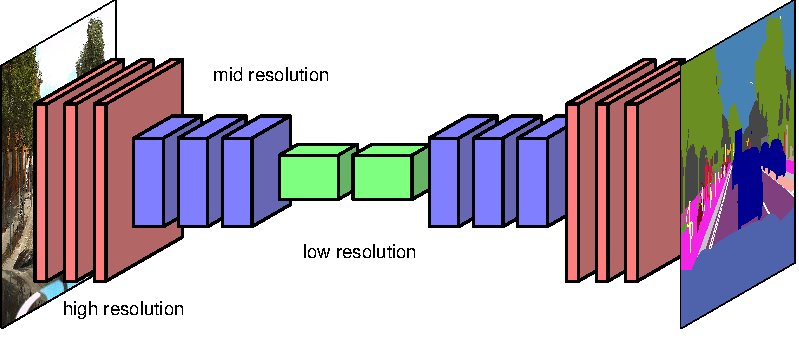
\includegraphics[width=0.72\linewidth]{Bishop10_27}
  \end{center}
  \figcap[0.97]{A segmentation network: strided convolutions and
  pooling reduce the feature maps to low resolution, then transpose
  convolutions and unpooling bring them back to the size of the image.
  Bishop \& Bishop (2024), Fig.~10.27.}
\end{frame}

\begin{frame}{Undoing pooling}
  \vspace{-0.3em}
  \begin{propx}[Unpooling inverts pooling]\label{th:unpool}
    \small
    Let $\mathbf{z}$ be a map and $2 \times 2$ blocks the pooling unit.
    \emph{Duplication} copies each value into its block, and
    average-pooling the result returns $\mathbf{z}$. \emph{Max-unpooling}
    puts each value into one cell of its block and zeros elsewhere, and
    max-pooling the result returns $\mathbf{z}$. If the cell chosen is the
    one that held the maximum when the map was pooled, the position of
    the maximum survives the round trip as well.
  \end{propx}
  \vspace{0.15em}
  {\footnotesize
  \begin{itemize}\itemsep0.22em
    \item Both are fixed functions with no parameters, like the
          poolings they undo; Class 23 drew them as circles
    \item The remembered positions are the first place spatial
          information is handed \alert{across} the bottleneck instead
          of through it
  \end{itemize}}
  \srcline{Bishop \& Bishop (2024), \S10.5.2, Figs.~10.28--10.29;
  Badrinarayanan et al.\ (2015).}
\end{frame}

\begin{frame}{Unpooling, drawn}
  \vspace{-0.3em}
  \begin{center}
    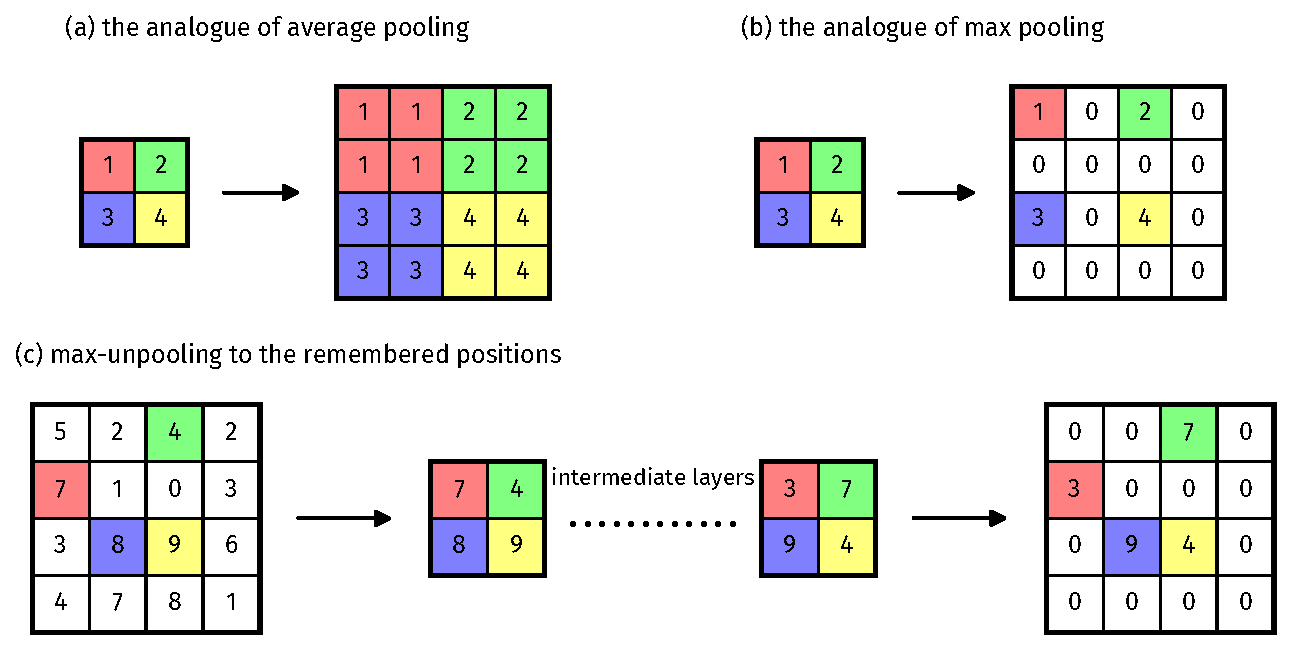
\includegraphics[width=0.74\linewidth]{unpooling}
  \end{center}
  \vspace{-0.7em}
  {\tiny\color{mcMuted}
  (a) the analogue of average pooling copies each value into its block;
  (b) the analogue of max pooling puts it in the first cell and zeros
  elsewhere. (c) remembering where each maximum was: the $4 \times 4$
  array is max-pooled, passes through intermediate layers, and is
  unpooled with each value at the position its maximum came from. Every
  number is computed by the pooling functions.
  \hfill Bishop \& Bishop (2024), Figs.~10.28 and 10.29.\par}
\end{frame}

\begin{frame}{Learned up-sampling}
  \vspace{-0.3em}
  \begin{propx}[Transpose convolution]\label{th:tconv}
    \small
    Write a strided convolution with no padding as a matrix, so the
    down-sampled map is $\mathbf{z} = \mathbf{M}\mathbf{x}$. The up-sampling in
    which each unit of $\mathbf{z}$ multiplies the kernel into a patch of
    the output, patches stepping by the stride and overlaps summed, is
    exactly $\mathbf{M}^{\mathsf T}\mathbf{z}$.
  \end{propx}
  \vspace{0.05em}
  {\footnotesize
  \begin{itemize}\itemsep0.26em
    \item \focus{1}{Proof. Row $r$ of $\mathbf{M}$ holds the kernel at the
          $r$-th window position, so column $q$ of $\mathbf{M}^{\mathsf T}$
          holds the same numbers, indexed by output pixel.}
    \item \focus{2}{$\mathbf{M}^{\mathsf T}\mathbf{z} = \sum_r z_r\,(\text{row } r)^{\mathsf T}$
          adds $z_r$ times the kernel at window position $r$: a
          scattered patch per unit, overlaps summed. \hfill $\square$}
    \item \focus{3}{The stride is now fractional --- one step in the
          input is two in the output --- and the kernel is
          \alert{learned}, unlike duplication. Call it neither
          ``deconvolution'', which means something else.}
  \end{itemize}}
  \srcline{Bishop \& Bishop (2024), \S10.5.3, Fig.~10.30, Exercise 10.13;
  Dumoulin \& Visin (2016).}
\end{frame}

\begin{frame}{Transpose convolution, drawn}
  \vspace{-0.3em}
  \begin{center}
    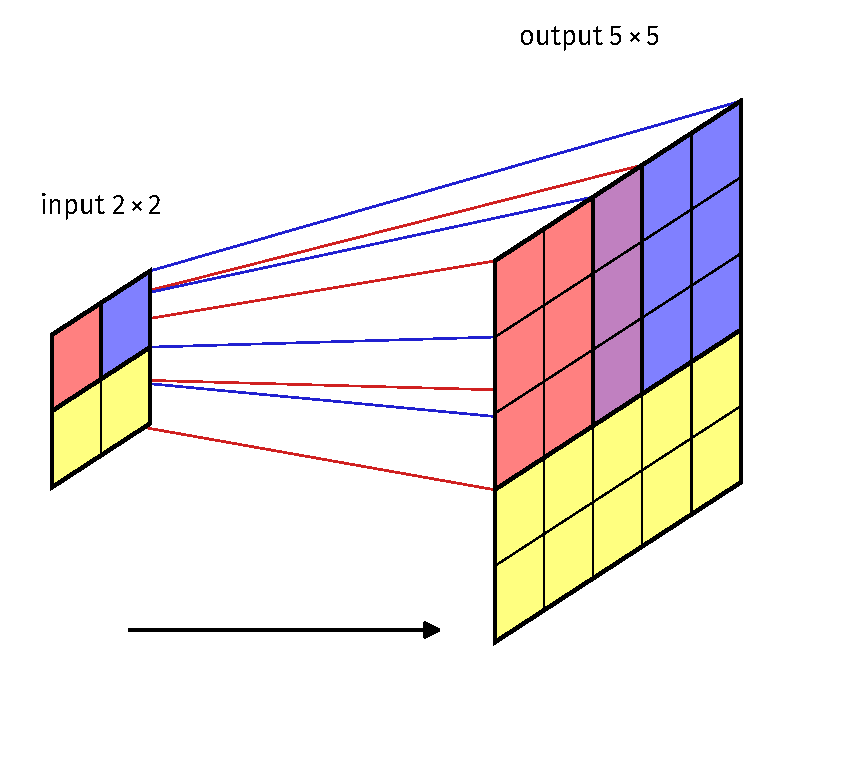
\includegraphics[height=0.62\textheight]{transpose_conv}
  \end{center}
  \vspace{-0.6em}
  {\tiny\color{mcMuted}
  A $3 \times 3$ kernel with an output stride of two: the red output
  patch is the kernel times the red input unit, the blue patch likewise,
  and where the patches overlap (purple) the contributions are summed.
  The build checks that this scattering equals $\mathbf{M}^{\mathsf T}\mathbf{z}$
  for the matrix of the $5 \times 5 \to 2 \times 2$ convolution.
  \hfill Bishop \& Bishop (2024), Fig.~10.30, Exercise 10.13.\par}
\end{frame}

\begin{frame}{Fully convolutional networks}
  \vspace{-0.3em}
  \begin{propx}[Any size in, the same size out]\label{th:fcn}
    \small
    A network of convolutions with same padding, poolings and
    transpose convolutions, with no fully connected layer and matched
    down- and up-sampling factors, is defined for an input of any
    height and width and returns a map of the same height and width.
  \end{propx}
  \vspace{0.15em}
  {\footnotesize
  \begin{itemize}\itemsep0.26em
    \item Every operation in it is local and weight-shared, so nothing
          in the parameters refers to the image size; only a fully
          connected layer does
    \item A $1 \times 1$ convolution at the end maps the channels to
          the $C$ classes and a softmax at every position finishes the
          job --- the fully connected head became convolutional too
    \item The encoder side is sometimes called the encoder and the
          up-sampling side the decoder; the shape gives the names
          hourglass and encoder--decoder
  \end{itemize}}
  \srcline{Bishop \& Bishop (2024), \S10.5.3; Long et al.\ (2015);
  Prince (2023), \S10.5.3.}
\end{frame}

\begin{frame}{An early segmentation network}
  \vspace{-0.2em}
  \begin{center}
    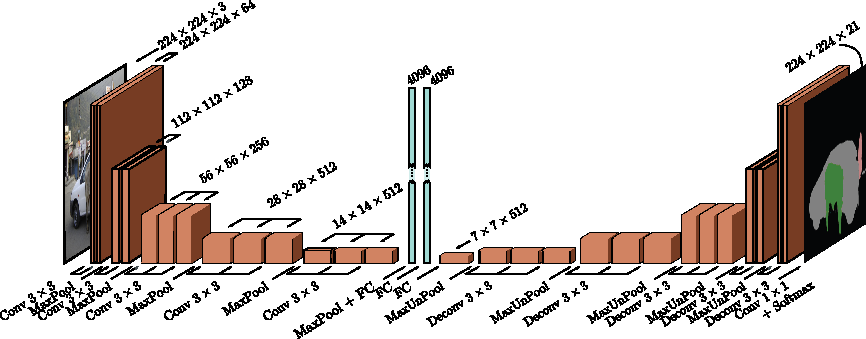
\includegraphics[width=0.80\linewidth]{P_ConvSemSeg}
  \end{center}
  \vspace{-0.2em}
  \figcap[0.97]{The network of Noh et al.\ (2015): a VGG encoder to
  $7 \times 7$, fully connected layers of $4096$, and a mirror-image
  decoder of max-unpooling and transposed convolutions to
  $224 \times 224 \times 21$. Prince (2023), Fig.~10.19.}
\end{frame}

\begin{frame}{What it produces}
  \begin{center}
    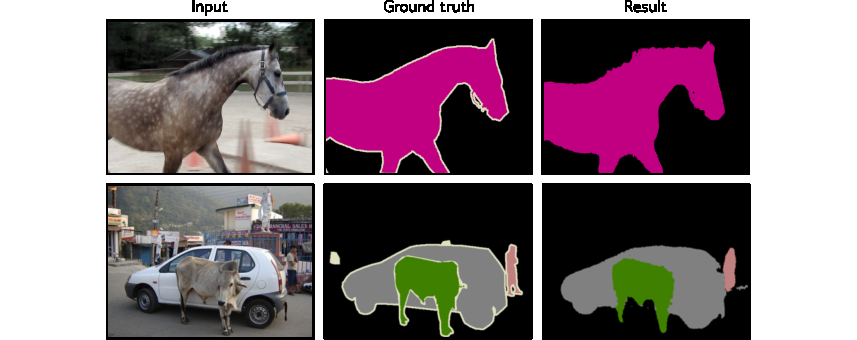
\includegraphics[width=0.80\linewidth]{P_ConvSemSegResults}
  \end{center}
  \vspace{-0.2em}
  \figcap[0.97]{From the $21$ probability maps, the most represented
  class is chosen greedily and its region inferred with a preference
  for connectedness; further classes are added while there is evidence.
  Prince (2023), Fig.~10.20, adapted from Noh et al.\ (2015).}
\end{frame}

\begin{frame}{What the bottleneck discards}
  \begin{center}
    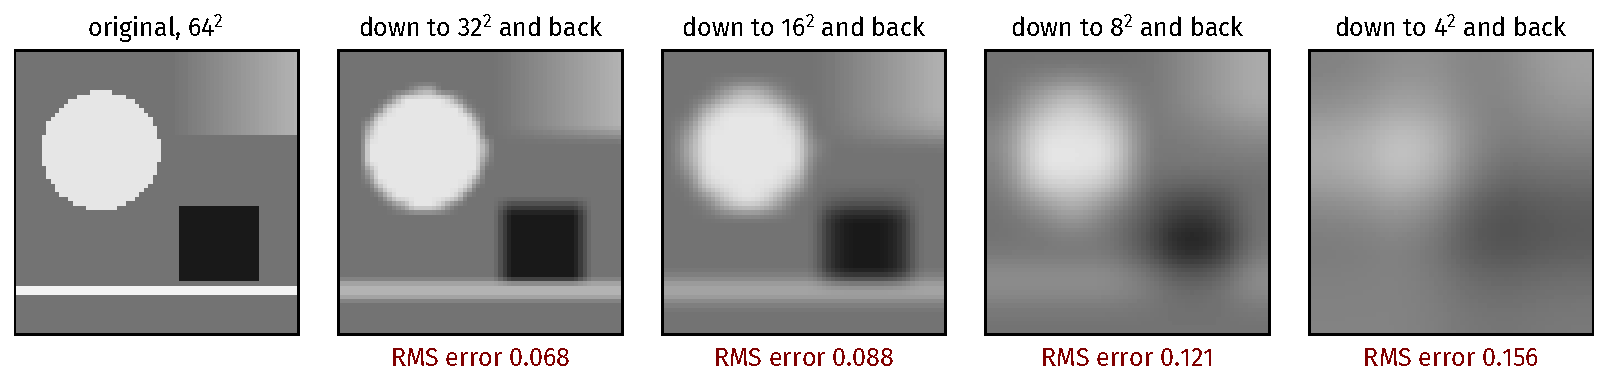
\includegraphics[width=0.88\linewidth]{downup}
  \end{center}
  \vspace{-0.2em}
  \figcap[0.97]{The scene of Class 23, average-pooled $L$ times and
  brought back by bilinear up-sampling: the error grows with depth, and
  the thin line is gone by the second level. Down-sampling discards
  positional information, which is fine for a label and a problem for a
  label per pixel.}
  \srcline{Bishop \& Bishop (2024), \S10.5.4.}
\end{frame}

\begin{frame}{The U-net}
  \begin{center}
    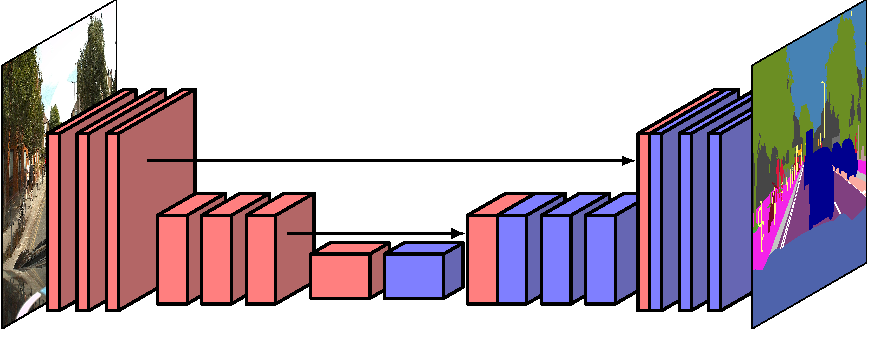
\includegraphics[width=0.80\linewidth]{Bishop10_31}
  \end{center}
  \vspace{-0.2em}
  \figcap[0.97]{A symmetrical arrangement of down-sampling and
  up-sampling layers; the output of each down-sampling layer is
  concatenated with the corresponding up-sampling layer, so the decoder
  reads coarse semantics from below and fine positions from the side.
  Bishop \& Bishop (2024), Fig.~10.31.}
\end{frame}

% =====================================================================
\section{Putting It Together}
% =====================================================================

\begin{frame}{Three tasks, one trunk}
  \vspace{0.2em}
  {\scriptsize
  \renewcommand{\arraystretch}{1.36}
  \begin{tabular}{@{}l@{\hspace{1.0em}}l@{\hspace{1.0em}}l@{\hspace{1.0em}}l@{}}
    & \textbf{classification} & \textbf{detection} & \textbf{segmentation}\\
    output & $C$ probabilities & boxes $+$ class $+$ score & $C$ probabilities per pixel\\
    symmetry wanted & invariance & equivariance of the box & equivariance of every pixel\\
    resolution & discarded & kept on a coarse grid & recovered in full\\
    head & fully connected $+$ softmax & grid of linear $+$ softmax & $1 \times 1$ conv $+$ softmax\\
    loss & cross-entropy & cross-entropy $+$ sum of squares & cross-entropy per pixel\\
    scored by & top-1, top-5 error & IoU $> 0.5$ & per-pixel accuracy\\
  \end{tabular}}
  \vspace{0.6em}

  \begin{redhighlight}
    The trunk is the same object in all three --- a convolutional stack
    that shrinks the map and grows the channels. What differs is how
    much of the map's resolution the head is allowed to keep.
  \end{redhighlight}
\end{frame}

\begin{frame}{Takeaways}
  \vspace{-0.1em}
  {\scriptsize
  \begin{enumerate}\itemsep0.22em
    \item Three tasks, three output structures: one distribution, a
          grid of boxes, a distribution per pixel; the structure decides
          what resolution the network may discard
    \item Classification wants invariance, so the trunk pools; depth,
          not width, was what took AlexNet to VGG (Definition~\ref{th:cls})
    \item A box is scored by intersection over union, a ratio in
          $[0, 1]$ (Definition~\ref{th:iou})
    \item Scanning a classifier is itself a convolution, so all windows
          cost one enlarged pass (Proposition~\ref{th:slide})
    \item Non-max suppression turns many firings into one box per
          object; YOLO predicts the grid directly
          (Definition~\ref{th:yolo})
    \item Segmentation wants equivariance, so the resolution must come
          back: unpooling (Proposition~\ref{th:unpool}) and transpose
          convolution, which is literally $\mathbf{M}^{\mathsf T}$
          (Proposition~\ref{th:tconv})
    \item No fully connected layer means any image size in, the same
          size out (Proposition~\ref{th:fcn})
    \item Down-sampling discards positional information; the U-net
          hands the resolution across by concatenation
  \end{enumerate}}
  \bridge{Class 25 opens the trunk: how depth composes filters, which
  architectures became standard, and what a trained filter responds to.}
\end{frame}

\begin{frame}[allowframebreaks]{References}
  \vspace{0.3em}
  {\scriptsize
  \begin{enumerate}\itemsep0.30em
    \item C.\ M.\ Bishop \& H.\ Bishop, \emph{Deep Learning: Foundations
          and Concepts}, Springer, 2024. \S10.4 (Figs.~10.19--10.25,
          Exercise 10.12); \S10.5 (Figs.~10.26--10.31, Exercise 10.13).
    \item S.\ J.\ D.\ Prince, \emph{Understanding Deep Learning}, MIT
          Press, 2023. \S10.5 (Figs.~10.15--10.21).
    \item A.\ Krizhevsky, I.\ Sutskever \& G.\ E.\ Hinton, ``ImageNet
          classification with deep convolutional neural networks'',
          NeurIPS 2012.
    \item K.\ Simonyan \& A.\ Zisserman, ``Very deep convolutional
          networks for large-scale image recognition'', ICLR 2015.
    \item O.\ Russakovsky et al., ``ImageNet large scale visual
          recognition challenge'', \emph{IJCV} 115, 2015.
    \item P.\ Sermanet et al., ``OverFeat: integrated recognition,
          localization and detection using convolutional networks'',
          ICLR 2014 (arXiv 2013).
    \item J.\ Redmon, S.\ Divvala, R.\ Girshick \& A.\ Farhadi, ``You
          only look once: unified, real-time object detection'',
          CVPR 2016.
    \item R.\ Girshick, ``Fast R-CNN'', ICCV 2015; S.\ Ren, K.\ He,
          R.\ Girshick \& J.\ Sun, ``Faster R-CNN'', NeurIPS 2015.
    \item J.\ Long, E.\ Shelhamer \& T.\ Darrell, ``Fully convolutional
          networks for semantic segmentation'', CVPR 2015.
    \item H.\ Noh, S.\ Hong \& B.\ Han, ``Learning deconvolution network
          for semantic segmentation'', ICCV 2015.
    \item V.\ Badrinarayanan, A.\ Kendall \& R.\ Cipolla, ``SegNet'',
          \emph{IEEE TPAMI} 39(12), 2017 (arXiv 2015).
    \item O.\ Ronneberger, P.\ Fischer \& T.\ Brox, ``U-Net: convolutional
          networks for biomedical image segmentation'', MICCAI 2015.
    \item V.\ Dumoulin \& F.\ Visin, ``A guide to convolution arithmetic
          for deep learning'', arXiv:1603.07285, 2016.
  \end{enumerate}}
\end{frame}

\begin{frame}[standout]
  Questions?
\end{frame}

\end{document}
